\documentclass[11pt,xcolor={dvipsnames},aspectratio=159,hyperref={pdftex,pdfpagemode=UseNone,hidelinks,pdfdisplaydoctitle=true},usepdftitle=false]{beamer}
\usepackage{presentation}[aspectratio=169]
\usepackage{math}
\usepackage{mathtools}
\usepackage{amsmath}
\usepackage{mleftright}

% Enter title of presentation PDF:
\hypersetup{pdftitle={Debt Sustainability I}}
% Enter link to PDF file with figures:


\begin{document}
% Enter presentation title:
\title{Debt Sustainability I}
\subtitle{Fiscal and Monetary Policy 2024}
% Enter presentation information:

% Enter presentation authors:
\author{Piotr Żoch}%
% Enter presentation location and date (optional; comment line if not needed):
\frame{\titlepage}

% Fill out content of presentation:
\begin{frame}{Plan}
    \begin{itemize}
    \item We review several approaches to debt sustainability analysis.
    \item Can the government service its current outstanding debt? Or will a fiscal consolidation be needed?
    \item Is the outstanding public debt and its projected path consistent with those of the government's revenues and expenditures?
   
    \end{itemize}
\end{frame}


\begin{frame}
    \heading{Classic Debt Sustainability Analysis}
\end{frame}

\begin{frame}{Debt to output ratio}

    \begin{itemize}
        \item The government static budget constraint is 
        \begin{align*}
            B_{t} = (1+r_{t})B_{t-1} + G_t - T_t.
        \end{align*}
        where $B_{t-1}$ is the \alb{market value} of all outstanding debt (all maturities), $G_t$ is nominal government spending (net of interest expenses), $T_t$ is nominal tax revenue, and $r_t$ is net nominal return on government debt.
        \item We abstract from money growth (we can treat money as a type of government debt).
        \item Note: it is often called ``flow budget constraint''. 
        \item Note: is it really a ``constraint''?
    \end{itemize}
\end{frame}
\begin{frame}{Debt to output ratio}

    \begin{itemize}
        \item Divide by \al{nominal} GDP $Y_t$ and rearrange  to get
        \begin{align*}
            \frac{B_{t}}{Y_t} = (1+r_{t})\frac{B_{t-1}}{Y_{t-1}}\frac{Y_{t-1}}{Y_t} + \frac{G_t}{Y_t} - \frac{T_t}{Y_t}.
        \end{align*}
        \item Define $$R_{t-j,t} \coloneq \prod_{k=1}^{j} \bp{1+r_{t-j+k}},$$ the cumulative return on debt from $t-j$ to $t$.
        \item Define $$X_{t-j,t} \coloneq \prod_{k=1}^{j} \frac{Y_{t-j+k}}{Y_{t-j+k-1}},$$ the cumulative gross growth rate of GDP from $t-j$ to $t$.
        
    \end{itemize}
\end{frame}

\begin{frame}{Debt to output ratio}

    \begin{itemize}
        \item For simplicity assume $B_0=0$.
        \item We can write the debt to output ratio as 
        \begin{align*}
            \frac{B_{t}}{Y_t} = \sum_{j=0}^t \frac{G_{t-j}-T_{t-j}}{Y_{t-j}} \frac{R_{t-j,t}}{X_{t-j,t}}
        \end{align*}
        \item Debt to output ratio today is determined by: 
        \begin{enumerate}
            \item The past primary deficits to GDP ratios;
            \item The past returns on debt;
            \item The past growth rates of (nominal) GDP.
        \end{enumerate}
        \item We can use the formula above to understand what determines the current debt to output ratio. 
    \end{itemize}
\end{frame}

\begin{frame}{Classic Debt Sustainability Analysis}
    \begin{itemize}
        \item A version of the formula is often used to assess \al{debt sustainability} -- "whether the government can service its debt".
        \item \alr{Warning}: this is about the future, not the present. The fact that people use the formula to assess the current situation is often a red flag!
        \item Classic debt sustainability analysis looks at the "long run".
        \end{itemize}
\end{frame}


\begin{frame}{Classic Debt Sustainability Analysis}
    \begin{itemize}
        \item Assume that the economy is in a steady state with a constant growth rate of GDP $X$, a constant rate of return $R$ and a constant primary deficit to GDP ratio.
        \item What is the debt to output ratio consistent with the above?
        \item If the observed current debt to output ratio is \al{below} this level, it is \al{sustainable}.
    \end{itemize}
\end{frame}

\begin{frame}{Classic Debt Sustainability Analysis}

    \begin{itemize}
        \item Classic debt sustainability analysis usually analyzes deterministic setups (or perfect foresight).
        \item In these setups, the appropriate $R$ is the \alb{risk-free rate}, $R^f$. 
        \item Assuming the above, the formula in the steady state becomes 
        \begin{align*}
            \frac{B}{Y} = \frac{G-T}{Y}\frac{X}{X-R^f}.
        \end{align*}
        \item For simplicity define $x\coloneqq X - 1$ and $r^f\coloneqq R^f - 1$ so we have         
        \begin{align*}
            \frac{B}{Y} = \frac{G-T}{Y}\frac{1+x}{x-r^f}.
        \end{align*}
        \item Hote: here $X$ and $R$ are one period rates (not cumulative). 
    \end{itemize}
\end{frame}

\begin{frame}{Classic Debt Sustainability Analysis}
    \begin{align*}
        \frac{B}{Y} = \frac{G-T}{Y}\frac{1+x}{x-r^f}
    \end{align*}
    \begin{itemize}
        \item Example: the Treaty of Maastricht set the limit of the debt to output ratio at 60\% and the deficit to output ratio at 3\%. What must be the growth rate of GDP and the risk-free rate for this to be sustainable?
        \end{itemize}
\end{frame}

\begin{frame}{Classic Debt Sustainability Analysis}
    \begin{align*}
        \frac{B}{Y} = \frac{G-T}{Y}\frac{1+x}{x-r^f}
    \end{align*}
    \begin{itemize}
        \item For $B\slash Y = 0.6$ and $G-T\slash Y = 0.03$ we have $\frac{0.6}{0.03} = 20$.
        \item We get $\frac{1+x}{x-r^f} = 20$.
        \item For small $x$ we have $x\approx r^f + 0.005$, so the economy has to grow at 0.5\% above the risk-free rate per year for the debt at the limit to be sustainable with the largest allowed deficit.
        \item If the actual growth rate is lower, the debt to output ratio will be larger, even if the deficit is at the limit.
    \end{itemize}
\end{frame}



\begin{frame}{Classic Debt Sustainability Analysis}
    \begin{align*}
        \frac{B}{Y} = \frac{G-T}{Y}\frac{1+x}{x-r^f}
    \end{align*}
    \begin{itemize}
        \item The key role of $x-r^f$.
        \item Depending on the sign of $x-r^f$ you require either surpluses or deficits to keep the debt to output ratio constant.
        \begin{itemize}
            \item If $x<r^f$ you need surpluses.
            \item If $x>r^f$ you can have deficits.
        \end{itemize}
        \item A big "r versus g" debate (we have $x$ instead of $g$). 
    \end{itemize}
\end{frame}

\begin{frame}{Classic Debt Sustainability Analysis}
    \begin{itemize}
        \item If $x>r^f$ it seems there is \al{no fiscal cost} to debt.
        \item Blanchard (2019) argues that $x>r^f$ is a norm, not an exception. 
        \item But what is $r^f$? How to measure it? Blanchard (2019) looks at the 1-year US Treasury bill rate, the 10-year US Treasury bond rate, adjusts for various maturities... 
        \item Note: it does not necessarily mean that it is \alb{optimal} to have deficits.
    \end{itemize}
\end{frame}

\begin{frame}{Rates in the US}
    \begin{figure}
        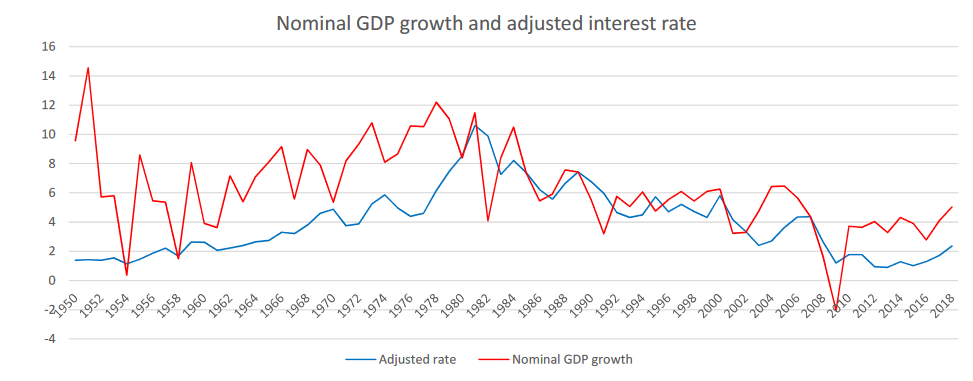
\includegraphics[width=1\textwidth]{blanchard_rg.png}
        \caption{Source: Blanchard (2019)}
    \end{figure}
   \end{frame}

\begin{frame}{Classic Debt Sustainability Analysis}
    \begin{itemize}
        \item It only \al{defines} what long-run debt
        is for a given long-run primary balance (or vice versa) \al{if} stationarity holds, or defines lower bounds on the
        short-run dynamics of the primary balance.
        \item It does not connect the outstanding initial debt of a
        particular period with the steady state.
        \item There might be multiple paths of debt that do not violate the \alb{intertemporal government budget constraint} (IGBC), some of them can even go to infinity (but slowly enough)!
        \item IGBC: the value of debt is equal to the present discounted value of future primary surpluses.
    \end{itemize}
\end{frame}

\begin{frame}
    \heading{Intertemporal Government Budget Constraint}
\end{frame}

\begin{frame}{IGBC}
    \begin{itemize}
        \item We used the government budget constraint by solving it \al{backward} (go back in time).
        \item We can also solve it \al{forward} -- the \alb{valuation approach}, the market value of government debt is determined by the discounted value of future government surpluses. 
        \item This idea is often used in finance (e.g., Campbell and Shiller 1988) - what determines stock prices?
        \item Allows us to think seriously about risk and asset pricing.
    \end{itemize}
\end{frame}

\begin{frame}{IGBC}
    \begin{itemize}
        \item Ignore risk for now and rewrite \begin{align*}             
            B_{t+1} = (1+r_{t+1})B_{t} + G_{t+1} - T_{t+1} \end{align*}
            as 
            \begin{align*}
                B_t =  \frac{1}{1+r_{t+1}}\bp{B_{t+1} - G_{t+1} + T_{t+1}}.
            \end{align*}
            \item Continue this process to get 
            \begin{align*}
                B_t = \sum_{j=1}^T \frac{1}{\prod_{k=1}^j (1+r_{t+k})} \bp{T_{t+j}-G_{t+j}} +\frac{1}{\prod_{k=1}^T (1+r_{t+k})}  B_{t+T}.
            \end{align*}
    \end{itemize}
\end{frame}

\begin{frame}{IGBC}
    \begin{itemize}
        \item Note: there is a term $\frac{1}{\prod_{k=1}^T (1+r_{t+k})}  B_{t+T}$. 
        \item If this term does not vanish as $T\to\infty$, there is a \al{bubble}.
        \item Imposing the no-Ponzi game condition ($\lim_{T\rightarrow \inf} \frac{1}{\prod_{k=1}^T (1+r_{t+k})}  B_{t+T} = 0$) on the above budget constraint, we get the IGBC: \begin{align*}
            B_t = \sum_{j=1}^\infty \frac{1}{\prod_{k=1}^j (1+r_{t+k})} \bp{T_{t+j}-G_{t+j}}.
        \end{align*}
        \item If the above is satisfied, we say that IGBC holds. 
        \end{itemize}
\end{frame}



\begin{frame}{IGBC}
    \begin{itemize}
        \item In a more general version IGBC is \begin{align*}
            B_t = \E_t \sum_{j=1}^\infty M_{t,t+j} \bp{T_{t+j}-G_{t+j}}
        \end{align*}
        \item We call $M_{t,t+j}$ the \alb{stochastic discount factor} (SDF). 
        \item It reflects how holders of government debt value discount future cash flows. 
        \item Generally it is a function of the state of the economy at time $t$ and $t+j$. Recall the first order condition for the household problem in the models we saw.
        \item We call the formula above the \alg{intertemporal government budget constraint} (IGBC).
        \end{itemize}
\end{frame}

\begin{frame}{Debt sustainability}
    \begin{itemize}
        \item We can say that debt is sustainable if and only if the IGBC holds.
        \item \al{Problem}: this condition is about the entire future. 
        \item \alb{Solution (?)}: use forecasts of future taxes and spending to compute the present value of future surpluses. Some early papers did this, but they used \alr{risk-free} rates.  
        \item Valid if one of these conditions holds: 
        \begin{enumerate}
            \item There is perfect foresight;
            \item Investors are risk-neutral;
            \item Primary surpluses do not covary with the SDF.
        \end{enumerate}
    \end{itemize}
\end{frame}


\begin{frame}{Bohn (1998)}
    \begin{itemize}
        \item Not even debt (or debt to GDP) going to infinity means that the IGBC does not hold, it has to go to infinity \al{slowly enough}.
        \item Bohn (1998): see if the government does something that guarantees the IGBC holds, investigate the \alb{fiscal reaction function}.
        \item Allows to sidestep the problem of forecasting future taxes and spending and choosing the correct discount rate.
        \item Sufficient condition: IGBC might also hold if it is violated, but if it is satisfied, IGBC holds for sure.
    \end{itemize}
\end{frame}

\begin{frame}{Bohn (1998)}
    \begin{itemize}
        \item Linear reaction function:
        \begin{align*}
            \frac{T_t - G_t}{Y_t} = \rho \frac{B_{t-1}}{Y_{t-1}} + Z_t + \epsilon_t
        \end{align*}
        \item The left hand side is \al{primary surplus}.
        \item $Z_t$ is a vector of exogenous variables that affect the primary surplus.
        \item Check if $\rho>0$ -- raise surplus if debt is high. 
        \item If $\rho>0$, then the \alb{IGBC holds} even if it is \alr{below} the interest rate (net of $x$).
    \end{itemize}
\end{frame}

\begin{frame}{Bohn (1998)}
    \begin{itemize}
        \item If $\rho>0$, the IGBC holds for \al{any} initial level of debt.
        \item This analysis works also for $r-x=0$ -- there was division by zero in the classic analysis.
        \item If $r-x>\rho>0$, debt explodes, but the IGBC \al{still} holds (under certain conditions: see Bohn 2007).
    \end{itemize}
\end{frame}

\begin{frame}{Bohn (1998)}
    \begin{itemize}
        \item Bohn (1998) estimates $\rho$ for the US in 1916-1995.
        \item He includes the level of temporary government spending and business cycle indicator in $Z_t$.
        \item He find a \al{positive} value of $\rho$, around 0.05 for the entire sample.
    \end{itemize}
\end{frame}

\begin{frame}{Bohn (1998)}
    \begin{figure}
        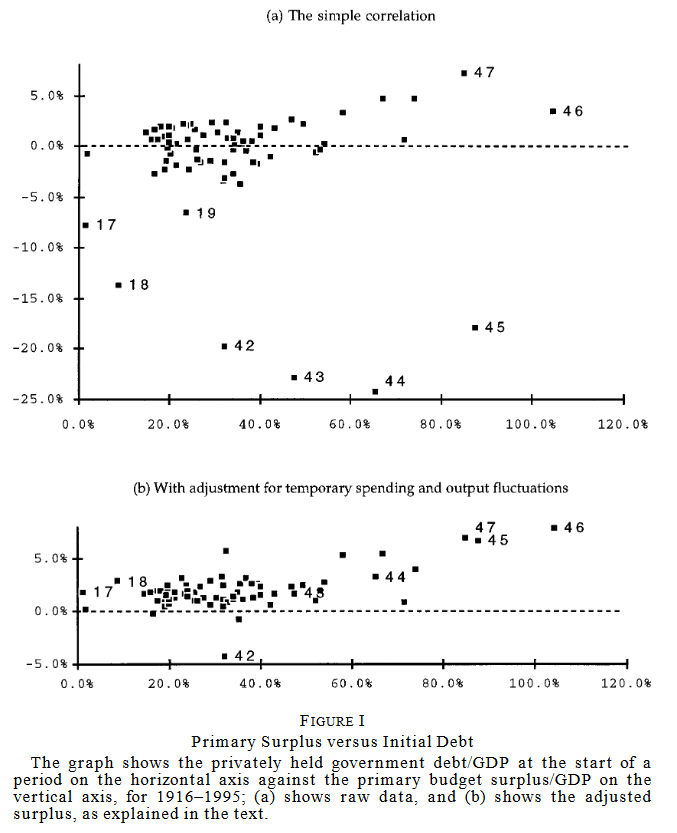
\includegraphics[width=0.5\textwidth]{bohn_1.png}
        \caption{Source: Bohn (1998)}
    \end{figure}
   \end{frame}

   \begin{frame}{Bohn (1998)}
    \begin{figure}
        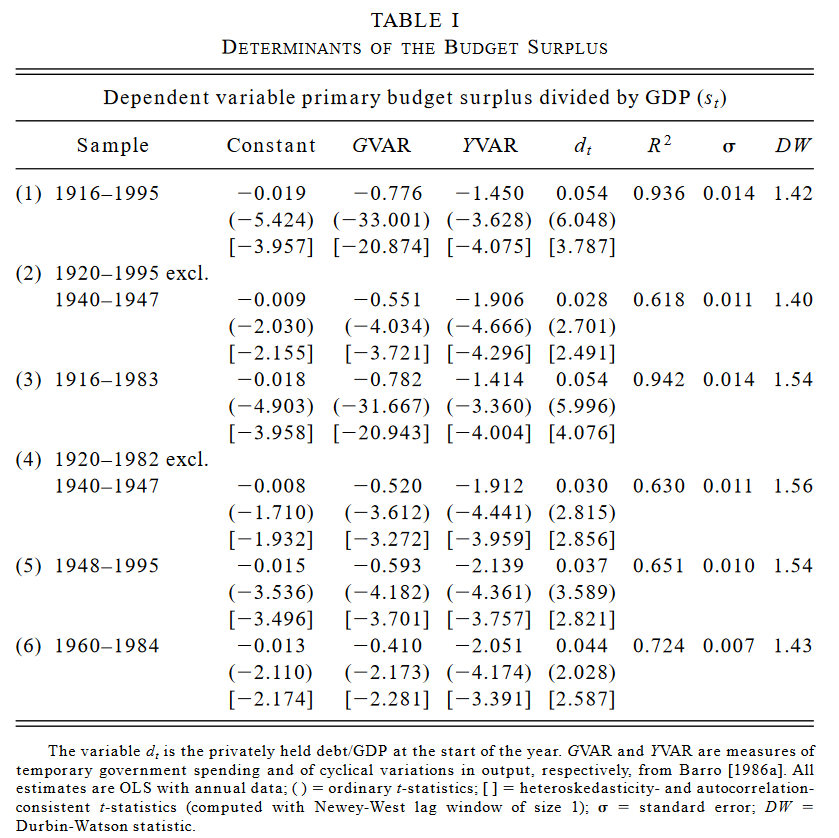
\includegraphics[width=0.5\textwidth]{bohn_2.png}
        \caption{Source: Bohn (1998)}
    \end{figure}
   \end{frame}

\begin{frame}{Fiscal reaction functions}
    \begin{itemize}
        \item Bohn (2008) extends the analysis to 1793-2003.
        \item He finds that $\rho>0.1$, more than twice as large as in the previous study.
        \item Mendoza and Ostry (2008) study fiscal reaction functions for a panel of multiple countries -- similar results.
        \item Ghosh et al. (2013) show that $\rho$ is much lower at high levels of debt. 
        \item D'Erasmo et al. (2016):
         \begin{enumerate}
            \item primary balance adjustment in the US after 2008 was \al{too large} to be explained by the fiscal reaction function;
            \item adjustment is \al{slower} than before (structural break);
            \item nevertheless, with the estimated $\rho$, the IGBC holds.
        \end{enumerate}
    \end{itemize}
\end{frame}

\begin{frame}{Fiscal reaction functions}
    \begin{itemize}
        \item Leeper (2017) warns against using surplus-debt regressions to assess debt sustainability.
        \item For the estimator of $\rho$ to be \alb{consistent}, we must have $$\E{\epsilon_t \mid \frac{B_{t-1}}{Y_{t-1}}} = 0.$$ \begin{enumerate}
            \item This means that shocks at $t-1$ that affect debt-output ratio in must not affect $\epsilon_t$.
            \item This means that the debt-output ratio cannot depend on the expectation of $\epsilon_t$.
        \end{enumerate}
        \item Since the value of debt depends on the expected value of future surpluses, this is a strong assumption: $\epsilon_t$ could be serially correlated.
    \end{itemize}
\end{frame}


\end{document}